\begin{frame}
 \frametitle{Outline}
 \tableofcontents
\end{frame}

\section{Fundamentals \\ \normalsize \textcolor{black!60!bgcolorAlt}{Algebras, Modules, Quivers}}

\begin{frame}{Algebras}
 \begin{alertblock}{$k$-algebra}
 	An algebra over a field $k$ is a $k$-vector space equipped with a
 	\alert{bilinear product}.
 \end{alertblock}
 \pause
 \textbf{Motivating examples}
 \begin{itemize}
  \item Complex numbers as the vector space $\R^2$ with the typical product of
   complex numbers.
  \pause
 	\item Ring of polynomials (over $k$) with polynomial multiplication.
 	\pause
 	\item Ring of square matrices with matrix multiplication.
 \end{itemize}
\end{frame}

\begin{frame}{Modules}
 \begin{alertblock}{$\Lambda$-module}
  Let $\Lambda$ be a $k$-algebra. A right $\Lambda$-module is a pair $(M, \cdot
  )$ where $M$ is a $k$-vector space and $ \cdot :M \times A \to M$ is a binary
  operation satisfying natural commutativity and associativity rules.
 \end{alertblock}
 \pause
 \textbf{Examples}
 \begin{itemize}
  \item Each algebra is a module (left or right) over itself.
  \pause 
 	 \item $k[x,y] = (k[x])[y]$ is a module (left or right) over $k[x]$.
 \end{itemize}
 \pause
 \begin{block}{Indecomposability (`prime' modules)}
 	A (right) $\Lambda$-module $M$ is \alert{indecomposable} if $M \neq 0$ and $M
 	= M_1 \oplus M_2$ implies that $M_1 = 0$ or $M_2 = 0$.
 \end{block}
\end{frame}

\begin{frame}{Module homomorphisms}
 \begin{alertblock}{$\Lambda$-module homomorphism}
 	A map $f:M \to N$ between two (right) $\Lambda$-modules $M$ and $N$ is a
 	$\Lambda$-module homomorphism if it's $k$-linear and respects $ \cdot $, that
 	is
 	\[
 	 f(m \cdot \lambda) = f(m) \cdot \lambda \text{ for } \lambda \in \Lambda, m
 	 \in M.
 	\]
 \end{alertblock}
 \pause
 \begin{block}{Section/retraction}
 	A $\Lambda$-module homomorphism $f:M \to N$ is
 	\vspace*{-\parskip}
 	\begin{itemize}
 	 \item a \alert{section} if $ \exists g: N \to M$ such that $g \circ f = 1_N$.
 	 \item a \alert{retraction} if $ \exists h: N \to M$ such that $f \circ h =
 	 	1_M$.
 	\end{itemize}
 \end{block}
\end{frame}

\begin{frame}[fragile]
 \frametitle{Module homomorphisms}
 \begin{block}{Irreducibility (`prime' homomorphisms)}
 	A $\Lambda$-module homomorphism $f:M \to N$ is \alert{irreducible} if
 	\begin{itemize}
 	 \item $f$ is neither a \textbf{section} nor a \textbf{retraction};
 	 \pause
 	 \item whenever $f = f_2 \circ f_1$, then $f_2$ is a retraction or $f_1$ is a
 	 	section.
 	\end{itemize}
 	We denote the $k$-vector space of irreducible homomorphisms $M \to N$ as
 	$\mathrm{Irr}(M,N)$.
 \end{block}
 \begin{figure}[h]
  \centering
  \begin{tikzcd}
   M \ar[rr, "f"] \ar[dr, "f_1"'] & & N \\
   															 & X \ar[ur, "f_2"'] &
  \end{tikzcd}
 \end{figure}
\end{frame}

\begin{frame}[fragile]
 \frametitle{Quivers}
 \begin{alertblock}{Quiver}
 	A \alert{quiver} is an oriented graph with multiple edges and loops.
 \end{alertblock}
 \pause
 \textbf{Examples}
 \begin{figure}[h]
  \centering
 	\begin{subfigure}[c]{.49\textwidth}
 	 \centering
	 \tikzset{every loop/.style={min distance=5mm,looseness=20}}
 	 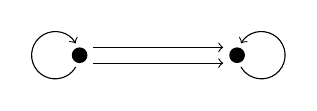
\begin{tikzpicture}
		\node[circle,fill,inner sep=2pt] (a) at (0,0) {};
		\node[circle,fill,inner sep=2pt] (b) at (2,0) {};
		\draw[->,shorten <=5pt,shorten >=5pt] (0, 0.1) -- (2, 0.1);
		\draw[->,shorten <=5pt,shorten >=5pt] (0, -0.1) -- (2, -0.1);
		\draw[<-] (-0.05,0.15) arc (30:330:0.3);
		\draw[<-] (2.05,0.15) arc (150:-150:0.3);
 	 \end{tikzpicture}
  \end{subfigure}
  \pause
 	\begin{subfigure}[c]{.49\textwidth}
 	 \centering
 	 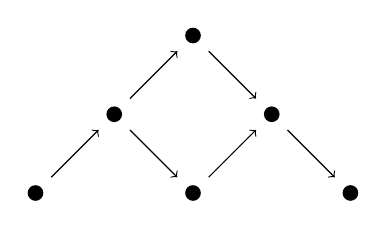
\begin{tikzpicture}
 	 	\node[circle,fill,inner sep=2pt] (a) at (0,0) {};
 	 	\node[circle,fill,inner sep=2pt] (b) at (1,1) {};
 	 	\node[circle,fill,inner sep=2pt] (c) at (2,0) {};
 	 	\node[circle,fill,inner sep=2pt] (d) at (2,2) {};
 	 	\node[circle,fill,inner sep=2pt] (e) at (3,1) {};
 	 	\node[circle,fill,inner sep=2pt] (f) at (4,0) {};

 	 	\draw[->,shorten <=5pt, shorten >=5pt] (a) -- (b);
 	 	\draw[->,shorten <=5pt, shorten >=5pt] (b) -- (c);
 	 	\draw[->,shorten <=5pt, shorten >=5pt] (b) -- (d);
 	 	\draw[->,shorten <=5pt, shorten >=5pt] (c) -- (e);
 	 	\draw[->,shorten <=5pt, shorten >=5pt] (d) -- (e);
 	 	\draw[->,shorten <=5pt, shorten >=5pt] (e) -- (f);
 	 \end{tikzpicture}
  \end{subfigure}
 \end{figure}
\end{frame}

\section{Auslander-Reiten Theory \\ \normalsize
\textcolor{black!60!bgcolorAlt}{Path Algebras, Representations, AR Quivers}}

\begin{frame}[fragile]
 \frametitle{Path algebras}
 \begin{alertblock}{The path algebra of a quiver}
  Let $Q$ be a quiver. The \alert{path algebra} $kQ$ of $Q$ is the $k$-algebra
  whose $k$-vector space has as its basis all paths of length $ \geq 0$ in $Q$
  and the product of two basis elements is the concatenation of paths.
 \end{alertblock}
\end{frame}

\begin{frame}[fragile]
 \frametitle{Path algebras -- Example}
 Consider the quiver
 \begin{figure}[h]
  \centering
  \begin{tikzpicture}
   \node[circle,fill,inner sep=2pt] (a) at (0,0) {};
   \node[circle,fill,inner sep=2pt] (b) at (2,0) {};
   \node[below=1mm of a] {$1$};
   \node[below=1mm of b] {$2$};
   \draw[->, shorten <=5pt, shorten >=5pt] (b) to node[above] {$a$} (a);
  \end{tikzpicture}
 \end{figure}

 \pause
 The basis of the path algebra $kQ$ is the triple $(e_1,e_2,a)$ (where $e_i$
 means `stay at $i$') and its multiplication table is
 \begin{table}[h]
  \centering
  \begin{tabular}{c|ccc}
   & $e_1$ & $e_2$ & $a$ \\
   \toprule
   $e_1$ & $e_1$ & $0$ & $0$\\
   $e_2$ & $0$ & $e_2$ & $a$\\
   $a$ & $a$ & $0$ & $0$
  \end{tabular}
 \end{table}

 \pause

 It's actually isomorphic to the $k$-algebra of lower triangular $2 \times 2$
 matrices over $k$.
\end{frame}

\begin{frame}
 \frametitle{Every algebra is a path algebra}
 \begin{theorem}
 	Let $k$ be an algebraically closed field and $\Lambda$ a basic, connected and
 	finite-dimensional algebra over $k$. Then there exists a finite connected
 	quiver $Q$ such that $\Lambda = kQ / I$ for some admissible ideal $I$ of $kQ$.
 \end{theorem}
 \pause
 \begin{theorem}[Gabriel's]
 	Let $\Lambda$ be as above. Then, $\Lambda$ is 
 \end{theorem}
\end{frame}

\begin{frame}{Integrals and Other Expressions}
	\begin{equation}
		\iint_{\partial\Omega}f(x)\diff{x} \in \complexes
	\end{equation}
	\begin{align}
		E &= mc^2\\
		F &= ma
	\end{align}

	\seprule
	
	\begin{tabular}{rl}
		$m$ & Mass\\
		$c$ & Speed of light
	\end{tabular}
\end{frame}
\begin{frame}{Theorems, Lemmas, ...}
	\begin{thm}
		The following statement is correct
		\begin{equation}
			\frac{\partial f(\vec{x})}{\partial x_i} = \sum_{l=1}^{L}\cos\left(l\frac{2\pi}{L} + 0\right)
		\end{equation}
	\end{thm}
\end{frame}

\section{Elements}

\begin{frame}[fragile]{Typography}
	\begin{verbatim}The theme provides sensible defaults to
		\emph{emphasize} text, \alert{accent} parts
		or show \textbf{bold} results.\end{verbatim}
	
	\begin{center}becomes\end{center}
	
	The theme provides sensible defaults to \emph{emphasize} text,
	\alert{accent} parts or show \textbf{bold} results.
\end{frame}

\begin{frame}{Font feature test}
	\begin{itemize}
		\item Regular
		\item \textit{Italic}
		\item \textsc{Small Caps}
		\item \textbf{Bold}
		\item \textbf{\textit{Bold Italic}}
		\item \textbf{\textsc{Bold Small Caps}}
		\item \texttt{Monospace}
		\item \texttt{\textit{Monospace Italic}}
		\item \texttt{\textbf{Monospace Bold}}
		\item \texttt{\textbf{\textit{Monospace Bold Italic}}}
	\end{itemize}
\end{frame}

\begin{frame}{Lists}
	\begin{columns}[T,onlytextwidth]
		\column{0.33\textwidth}
		Items
		\begin{itemize}
			\item Milk \item Eggs \item Potatoes
		\end{itemize}
		
		\column{0.33\textwidth}
		Enumerations
		\begin{enumerate}
			\item First, \item Second and \item Last.
		\end{enumerate}
		
		\column{0.33\textwidth}
		Descriptions
		\begin{description}
			\item[PowerPoint] Meeh. \item[Beamer] Yeeeha.
		\end{description}
	\end{columns}
\end{frame}
\begin{frame}{Tables}
	\begin{table}
		\caption{Largest cities in the world (source: Wikipedia)}
		\begin{tabular}{@{} lr @{}}
			\toprule
			City & Population\\
			\midrule
			Mexico City & 20,116,842\\
			Shanghai & 19,210,000\\
			Peking & 15,796,450\\
			Istanbul & 14,160,467\\
			\bottomrule
		\end{tabular}
	\end{table}
\end{frame}
\begin{frame}{Blocks}
	Three different block environments are pre-defined and may be styled with an
	optional background color.
	
	\begin{columns}[T,onlytextwidth]
		\column{0.45\textwidth}
		\begin{block}{Default}
			Block content.
		\end{block}
		
		\begin{alertblock}{Alert}
			Block content.
		\end{alertblock}
		
		\begin{exampleblock}{Example}
			Block content.
		\end{exampleblock}
		
		\column{0.45\textwidth}
		
		\metroset{block=fill}
		
		\begin{block}{Default}
			Block content.
		\end{block}
		
		\begin{alertblock}{Alert}
			Block content.
		\end{alertblock}
		
		\begin{exampleblock}{Example}
			Block content.
		\end{exampleblock}
		
	\end{columns}
\end{frame}
\begin{frame}{Line plots}
	\begin{figure}
		\begin{tikzpicture}
			\begin{axis}[
				betterplot,
				width=0.9\textwidth,
				height=6cm,
				]
				
				\addplot {sin(deg(x))};
				\addplot+[samples=100] {sin(deg(2*x))};
				
			\end{axis}
		\end{tikzpicture}
	\end{figure}
\end{frame}

\begin{frame}[standout,plain]
	Standout Frame!
\end{frame}


\appendix
\begin{frame}[fragile]{Backup slides}
	Sometimes, it is useful to add slides at the end of your presentation to
	refer to during audience questions.
	
	The best way to do this is to include the \verb|appendixnumberbeamer|
	package in your preamble and call \verb|\appendix| before your backup slides.
	
	The theme will automatically turn off slide numbering and progress bars for
	slides in the appendix.
\end{frame}
